\documentclass[tikz, margin=0.5cm]{standalone}
\usepackage[utf8x]{inputenc}
\usepackage{tikz}
\usepackage{xcolor}
\begin{document}
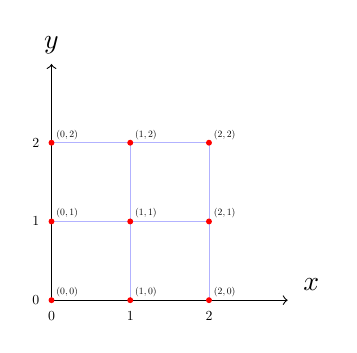
\begin{tikzpicture}
    \draw [->] (0, 0) -- (3, 0) node [near end, pos=1.1, above] {$x$};
    \draw [->] (0, 0) -- (0, 3) node [near end, pos=1, above] {$y$};
    
    \foreach \x in {0, 1, 2}{
        \draw (\x, -0.2) node [scale=0.5] {$\x$};
        \draw (-0.2, \x) node [scale=0.5] {$\x$};
    }

    \foreach \x in {1, 2}{
        \draw [color=blue!30, line width=0.1mm] (\x, 0) -- (\x, 2);
        \draw [color=blue!30, line width=0.1mm] (0, \x) -- (2, \x);
    }

    \foreach \x/\y in {0/0, 0/1, 0/2, 1/0, 1/1, 1/2, 2/0, 2/1, 2/2}{
        \draw [fill, color=red] (\x, \y) circle (0.03);
        \draw (\x+0.2, \y+0.1) node [scale=0.35] {$(\x, \y)$};
    }
    

    
\end{tikzpicture}
\end{document}